%%
%% This is file `sample-manuscript.tex',
%% generated with the docstrip utility.
%%
%% The original source files were:
%%
%% samples.dtx  (with options: `manuscript')
%%
%% IMPORTANT NOTICE:
%%
%% For the copyright see the source file.
%%
%% Any modified versions of this file must be renamed
%% with new filenames distinct from sample-manuscript.tex.
%%
%% For distribution of the original source see the terms
%% for copying and modification in the file samples.dtx.
%%
%% This generated file may be distributed as long as the
%% original source files, as listed above, are part of the
%% same distribution. (The sources need not necessarily be
%% in the same archive or directory.)
%%
%% Commands for TeXCount
%TC:macro \cite [option:text,text]
%TC:macro \citep [option:text,text]
%TC:macro \citet [option:text,text]
%TC:envir table 0 1
%TC:envir table* 0 1
%TC:envir tabular [ignore] word
%TC:envir displaymath 0 word
%TC:envir math 0 word
%TC:envir comment 0 0
%%
%%
%% The first command in your LaTeX source must be the \documentclass command. This is the generic manuscript mode required for submission and peer review.
\documentclass[manuscript,screen,review, language=greek, language=english]{acmart}
%% To ensure 100% compatibility, please check the white list of
%% approved LaTeX packages to be used with the Master Article Template at
%% https://www.acm.org/publications/taps/whitelist-of-latex-packages
%% before creating your document. The white list page provides
%% information on how to submit additional LaTeX packages for
%% review and adoption.
%% Fonts used in the template cannot be substituted; margin
%% adjustments are not allowed.
\usepackage[greek]{babel}
\usepackage{graphicx}
\graphicspath{{images/}}
\usepackage{hyperref}

%%
%% \BibTeX command to typeset BibTeX logo in the docs
\AtBeginDocument{%
  \providecommand\BibTeX{{%
	\normalfont B\kern-0.5em{\scshape i\kern-0.25em b}\kern-0.8em\TeX}}}

%%
%% For managing citations, it is recommended to use bibliography
%% files in BibTeX format.
%%
%% You can then either use BibTeX with the ACM-Reference-Format style,
%% or BibLaTeX with the acmnumeric or acmauthoryear sytles, that include
%% support for advanced citation of software artefact from the
%% biblatex-software package, also separately available on CTAN.
%%
%% Look at the sample-*-biblatex.tex files for templates showcasing
%% the biblatex styles.
%%
\bibliographystyle{acm-bib-format}

%%
%% end of the preamble, start of the body of the document source.
\begin{document}

%%
%% The "title" command has an optional parameter,
%% allowing the author to define a "short title" to be used in page headers.
\title{Εφαρμογή Αναζήτησης Ακινήτων}

%%
%% The "author" command and its associated commands are used to define
%% the authors and their affiliations.
%% Of note is the shared affiliation of the first two authors, and the
%% "authornote" and "authornotemark" commands
%% used to denote shared contribution to the research.
\author{Νικόλαος-Αλκίνοος Αλυσσανδράκης}
\email{alk.alyssandrakis@gmail.com}
\affiliation{%
  \institution{1072752}
  \streetaddress{}
  \city{}
  \state{}
  \country{}
  \postcode{}
}

\author{Δήμητρα-Μαρία Σκαμαντζούρα}
\email{dimiskama115@gmail.com}
\affiliation{%
  \institution{1072713}
  \streetaddress{}
  \city{}
  \country{}
}

\begin{abstract}
	Το θέμα του πρότζεκτ που ανατέθηκε στην ομάδα μας είναι η υλοποίηση μίας ιστοσελίδας
	αναζήτησης ακινήτων. Τα ακίνητα αυτά εμφανίζονται σε μορφή αγγελιών, όπου
	οποιοσδήποτε μπορεί να έχει πρόσβαση και να αναζητήσει με βάση τις επιθυμίες του.
	Στους χρήστες δίνεται η επιλογή δημιουργίας λογαριασμού, η οποία παρέχει τα προνόμια
	της προσθήκης αγγελιών στα αγαπημένα και την συγκρώτηση τους σε μία λίστα αγαπημένων
	στο προφίλ του χρήστη. Στις αγγελίες παρουσιάζονται τα στοιχεία του αγγελιοδότη και
	ο χρήστης μπορεί να έρθει σε επικοινωνία με τον αγγελιοδότη, εφόσον το επιθυμεί.
\end{abstract}


%%
%% This command processes the author and affiliation and title
%% information and builds the first part of the formatted document.
\maketitle

\section{Μεθοδολογια}

\subsection{Στόχος}
	Ο κύριος στόχος, κατά την υλοποίηση του πρότζεκτ, ήταν η πραγματοποίηση της κύριας
	αναζήτησης. Βασικά χαρακτηριστικά αυτής αποτελούσαν η περιοχή, το είδος ακινήτου, το
	εύρος της τιμής και του εμβαδού, καθώς επίσης το είδος της αγγελίας. Σε επόμενο
	στάδιο, επιθυμητό ήταν να προβάλλονταν στον χρήστη όλες οι αγγελίες ακινήτων που
	πληρούσαν τις προϋποθέσεις με όλες τις βασικές τους πληροφορίες.

\subsection{Υλοποίηση}

\subsubsection{Προσέγγιση}
	Πρώτο βήμα μετά την ανάθεση του θέματος ήταν να αναζητήσουμε αντίστοιχα παραδείγματα
	ιστοσελίδων και να κρίνουμε ποια χαρακτηριστικά θεωρούσαμε απαραίτητα για την
	ιστοσελίδα. Σε συνέχεια, υλοποιήσαμε το UI/UX design της εφαρμογής με χρήση του
	εργαλείου Figma και κανονίσαμε μία συνάντηση με τον κ. Αβούρη, προκειμένου να εκφέρει
	την
	αποψή του και να έχουμε το απαραίτητο feedback. Έχοντας αποκτήσει μία ξεκάθαρη
	εικόνα του περιεχομένου της ιστοσελίδας, προχωρήσαμε στον διαμοιρασμό της δουλειάς.
	Ο ένας ασχολήθηκε κατα κύριο λόγο με το Frontend (Σκαμανατζούρα Δήμητρα) και ο
	άλλος με το Backend (Αλκίνοος Αλυσσανδράκης).

\subsubsection{Εργαλεία \& Τεχνολογίες}
	Για την δημιουργία του front end τομέα της ιστοσελίδας αξιοποιήθηκαν οι εξής
	τεχνολογίες:

	\begin{itemize}
		\item Figma \cite{Figma}
		\item Handlebars \cite{Handlebars}
		\item CSS3 \cite{CSS}
		\item Javascript \cite{Javascript}
	\end{itemize}

	To handlebars εξηπυρετούσε τον σκοπό της ύπαρξης templates και την δυναμική
	δημιουργία των HTML που απευθύνονταν στον χρήστη.

	Αντίστοιχα για το κομμάτι του back end:

	\begin{itemize}
		\item Node.js \cite{Node.js}
		\item Express \cite{Express}
		\item express-handlebars \cite{express-handlebars}
		\item express-session \cite{express-session}
		\item MongoDB \cite{MongoDB}
		\item Mongoose \cite{Mongoose}
		\item Mockaroo \cite{Mockaroo}
		\item Docker \cite{Docker}
	\end{itemize}

	Για την καλύτερη συνεργασία ανάμεσα στους δύο συνεργάτες χρησιμοποιήθηκαν τα εξής
	εργαλεία:

	\begin{itemize}
		\item Git \cite{Git}
		\item GitHub
	\end{itemize}

	\subsection{Χρονοδιάγραμμα}
	Τα βήματα που πάρθηκαν χρονικά ήταν ως εξής:

	\begin{itemize}
		\item Ορισμός των βασικών χαρακτηριστικών της σελίδας
		\item Σχεδιασμός σελίδας στο χαρτί
		\item Σχεδιασμός σε Figma
		\item Υλοποίηση σελίδων με χρήση HTML και CSS
		\item Σχεδίαση της βάσης δεδομένων
		\item Υλοποίηση της βασικής λειτουργίας του backend
		\item Συμπλήρωση στοιχείων στη βάση δεδομένων
		\item Σύνδεση του backend με τη βάση δεδομένων
		\item Ολοκλήρωση της λειτουργικότητας της ιστοσελίδας
	\end{itemize}


\section{Frontend}
	Αρχικά, σε κάθε σελίδα υπάρχουν δύο βασικά στοιχεία, το λογότυπο της ιστοσελίδας μας
	και το εικονίδιο σύνδεσης χρήστη. Αν ο χρήστης κάνει κλικ πάνω στο εικονίδιο με το
	λογότυπο, τότε θα γίνει παραπομπή στην αρχική σελίδα, αν κάνει κλικ στο εικονίδιο
	χρήστη τότε θα εμφανιστεί το αντίστοιχο pop-up, αναλόγως αν είναι συνδεδεμένος ή όχι
	ο χρήστης. Η μορφή αυτών των pop-ups παρουσιάζεται στην εικόνα
	\emph{Fig. \ref{fig:pop-ups}}.

	\begin{figure}[H]
		   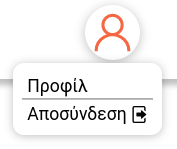
\includegraphics[width=0.2\textwidth]{pop-up_1.png}
		   
\includegraphics[width=0.15\textwidth]{pop-up_2.png}
		   \caption{Pop-ups}
		   \label{fig:pop-ups}
	\end{figure}

\subsection{Αρχική Σελίδα}
	Η πρώτη υλοποίηση, από άποψης frontend, ήταν η αρχική σελίδα της ιστοσελίδας.
	Έμπνευση για την συνολική εικόνα της ιστοσελίδας αποτέλεσαι κατά κύριο λόγo η σελίδα
	του σπιτόγατου (\href{www.spitogatos.gr}{Spitogatos}).
	Στη συνέχεια, βασική λογική της αρχικής σελίδας αποτελεί η επιλογή ενός εκ των δύο
	πιθανόν σεναρίων, ενοικίασης ή πώλησης, πριν ο χρήστης προχωρήσει στην
	αναζήτηση. Μπορεί επίσης να συμπληρώσει παραπάνω χαρακτηριστικά, όπως την περιοχή,
	την κατηγορία του ακινήτου κτλ.

	\begin{figure}[H]
		   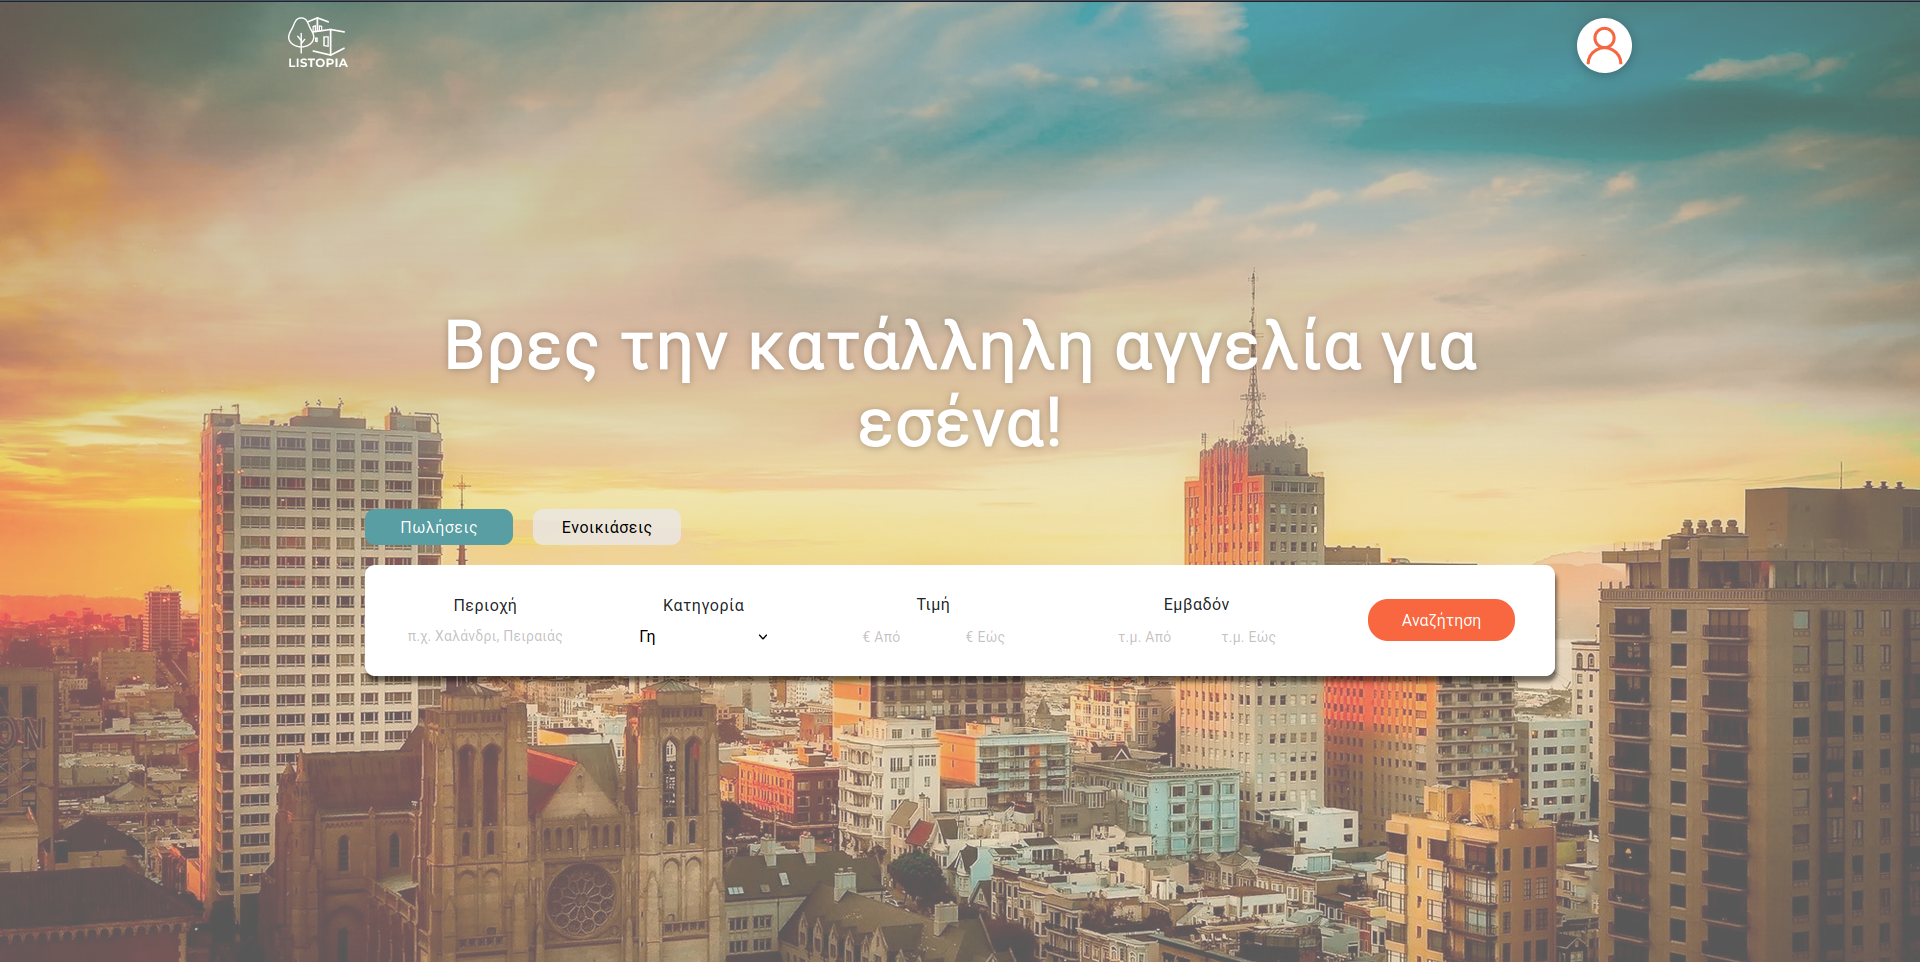
\includegraphics[width=0.8\textwidth]{home_page.png}
		   \caption{Αρχική Σελίδα}
		   \label{fig:home}
	\end{figure}

\subsection{Σελίδα Αναζήτησης}
	Η σελίδα προβολής των αποτελεσμάτων αναζήτησης είναι αναγκαία για την
	λειτουργικότητα της. Βασικό στοιχείο της υλοποίησης αποτελεί η προβολή των καρτών των
	αγγελιών που πληρούν τα χαρακτηριστικά που έχει δηλώσει ο χρήστης. Αυτές οι κάρτες
	αποτελούνται από μία εικόνα του ακινήτου, τα βασικά χαρακτηριστικά της αγγελίας,
	όπως τύπος, εμβαδόν, τιμή κλπ. Εφόσον ο χρήστης πατήσει κάποια από αυτές τις κάρτες,
	θα μεταφερθεί στην αντίστοιχη σελίδα της συγκεκριμένης αγγελίας. Επιπλέον, σε κάθε
	κάρτα υπάρχει η επιλογή τοποθέτησης της συγκεκριμένης αγγελίας στα αγαπημένα μέσω της
	καρδούλας που εμφανίζεται στην κάρτα. Λοιπά χαρακτηριστικά αυτής της σελίδας είναι η
	επιστροφή πίσω στην αρχική
	αλλά και η επιλογή φίλτρων αναζήτησης. Η μπάρα με τα φίλτρα εμφανίζεται πατώντας πάνω
	στο κουμπί που αναγράφει "Φίλτρα" και ξανακλείνει με τον ίδιο ακριβώς τρόπο.

	\begin{figure}[H]
		   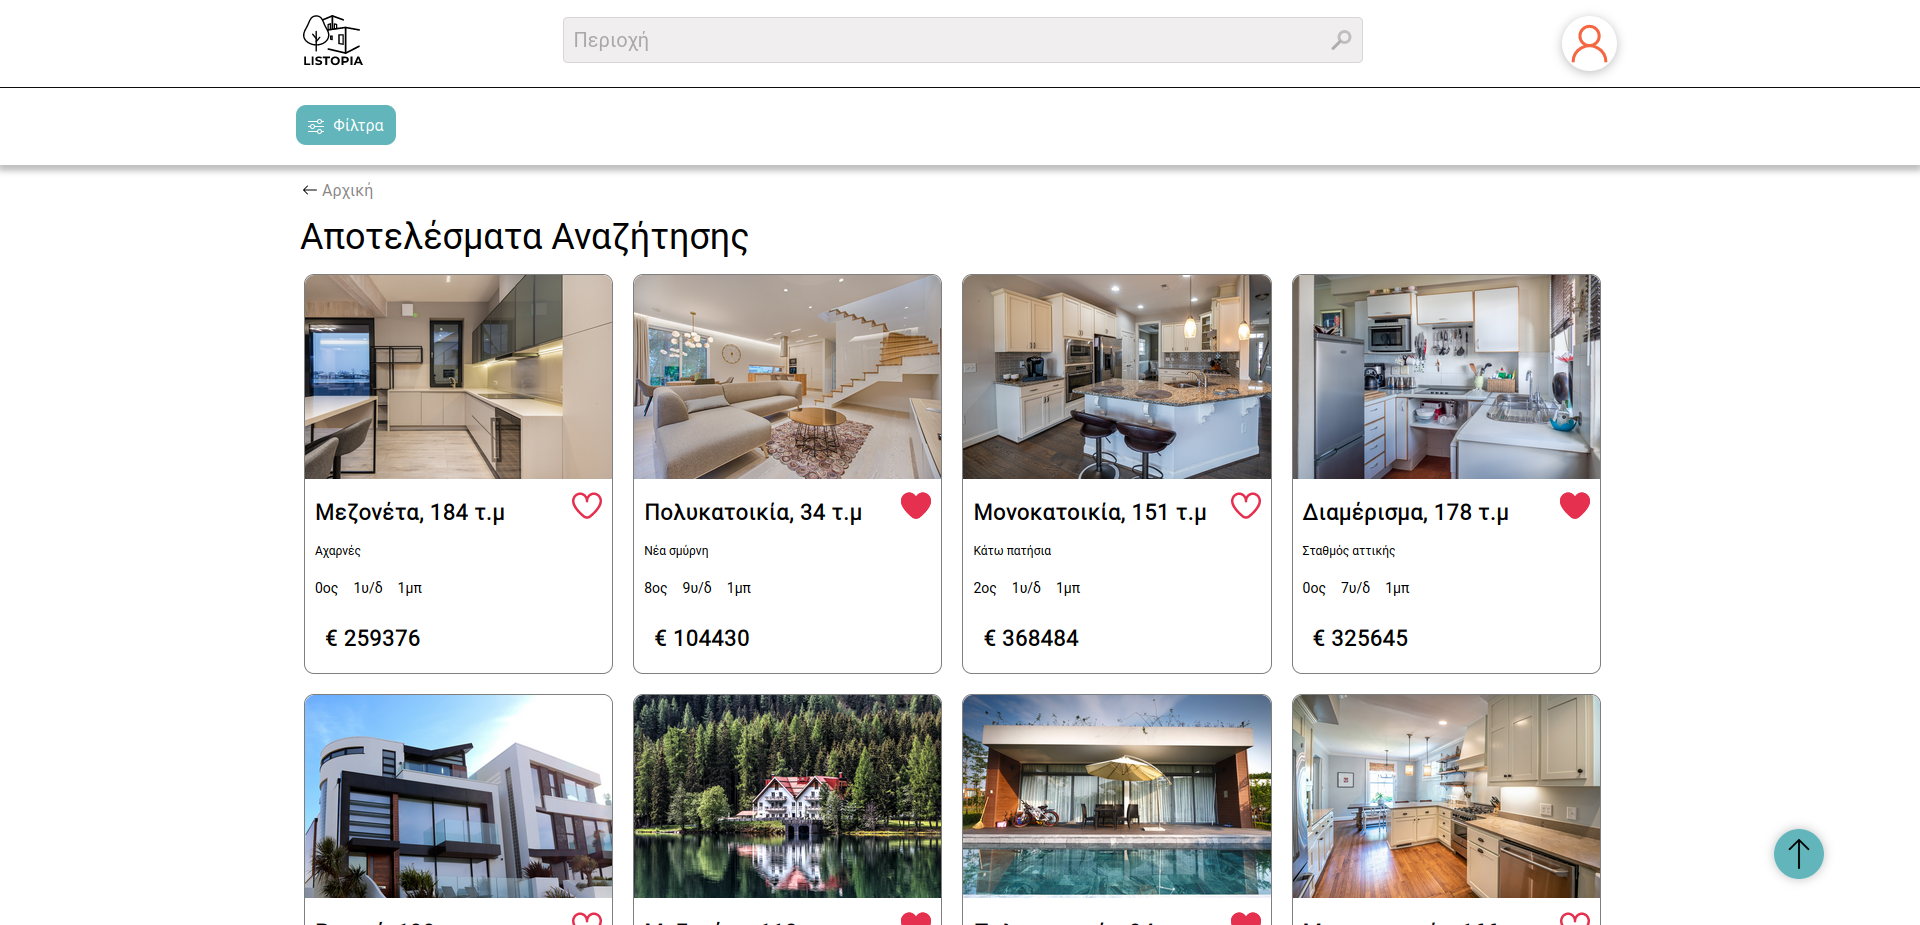
\includegraphics[width=0.8\textwidth]{search_page.png}
		   \caption{Αποτέλεσμα Αναζήτησης}
		   \label{fig:search_page}
	\end{figure}
	\begin{figure}[H]
		   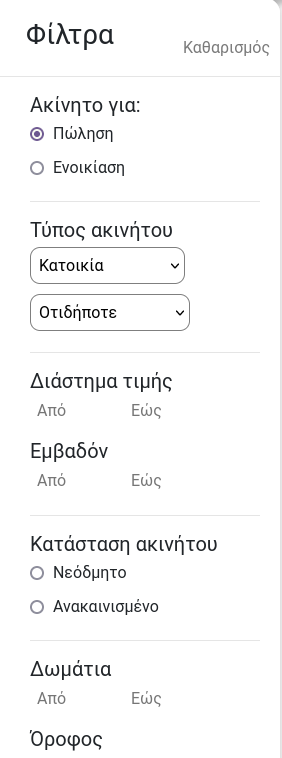
\includegraphics[width=0.2\textwidth]{filter1.png}
		   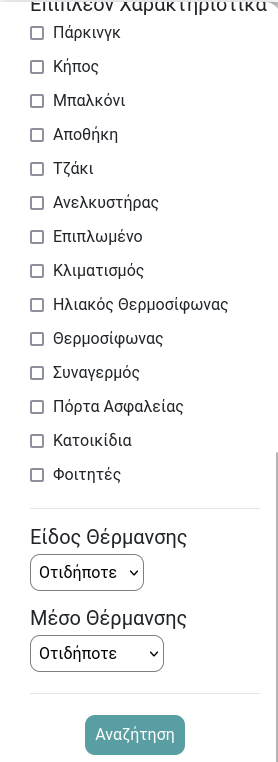
\includegraphics[width=0.2\textwidth]{filter2.png}
		   \caption{Φίλτρα}
		   \label{fig:filters}
	\end{figure}

\subsection{Σελίδα Αγγελίας}
	Κύριο χαρακτηριστικό της σελίδας αυτής αποτελεί ο τομέας των εικόνων. Οι εικόνες
	εμφανίζονται με την δομή που παρουσιάζεται στην εικόνα
	\emph{Fig. \ref{fig:listing_preview}} και
	σε περίπτωση που ο χρήστης πατήσει πάνω τους ανοίγει ένα pop-up carousel. Σε αυτό, ο
	χρήστης μπορεί να πλοηγηΘεί σε όλες τις διαθέσιμες εικόνες αυτού του ακινήτου όπως
	παρουσιάζεται στην εικόνα \emph{Fig. \ref{fig:carousel}}.
	Επιστρέφοντας στην αρχική όψη αυτής της σελίδας, ο χρήστης κάνοντας κύληση τη σελίδα
	προς τα
	κάτω μπορεί να ενημερωθεί για όλες τις λοιπές πληροφορίες για το συγκεκριμένο
	ακίνητο. Σε περίπτωση που ενδιαφέρεται, παρουσιάζονται τα στοιχεία επικοινωνίας του
	αγγελιοδότη και έτσι μπορεί να έρθει σε επικοινωνία μαζί του.

	\begin{figure}[H]
		   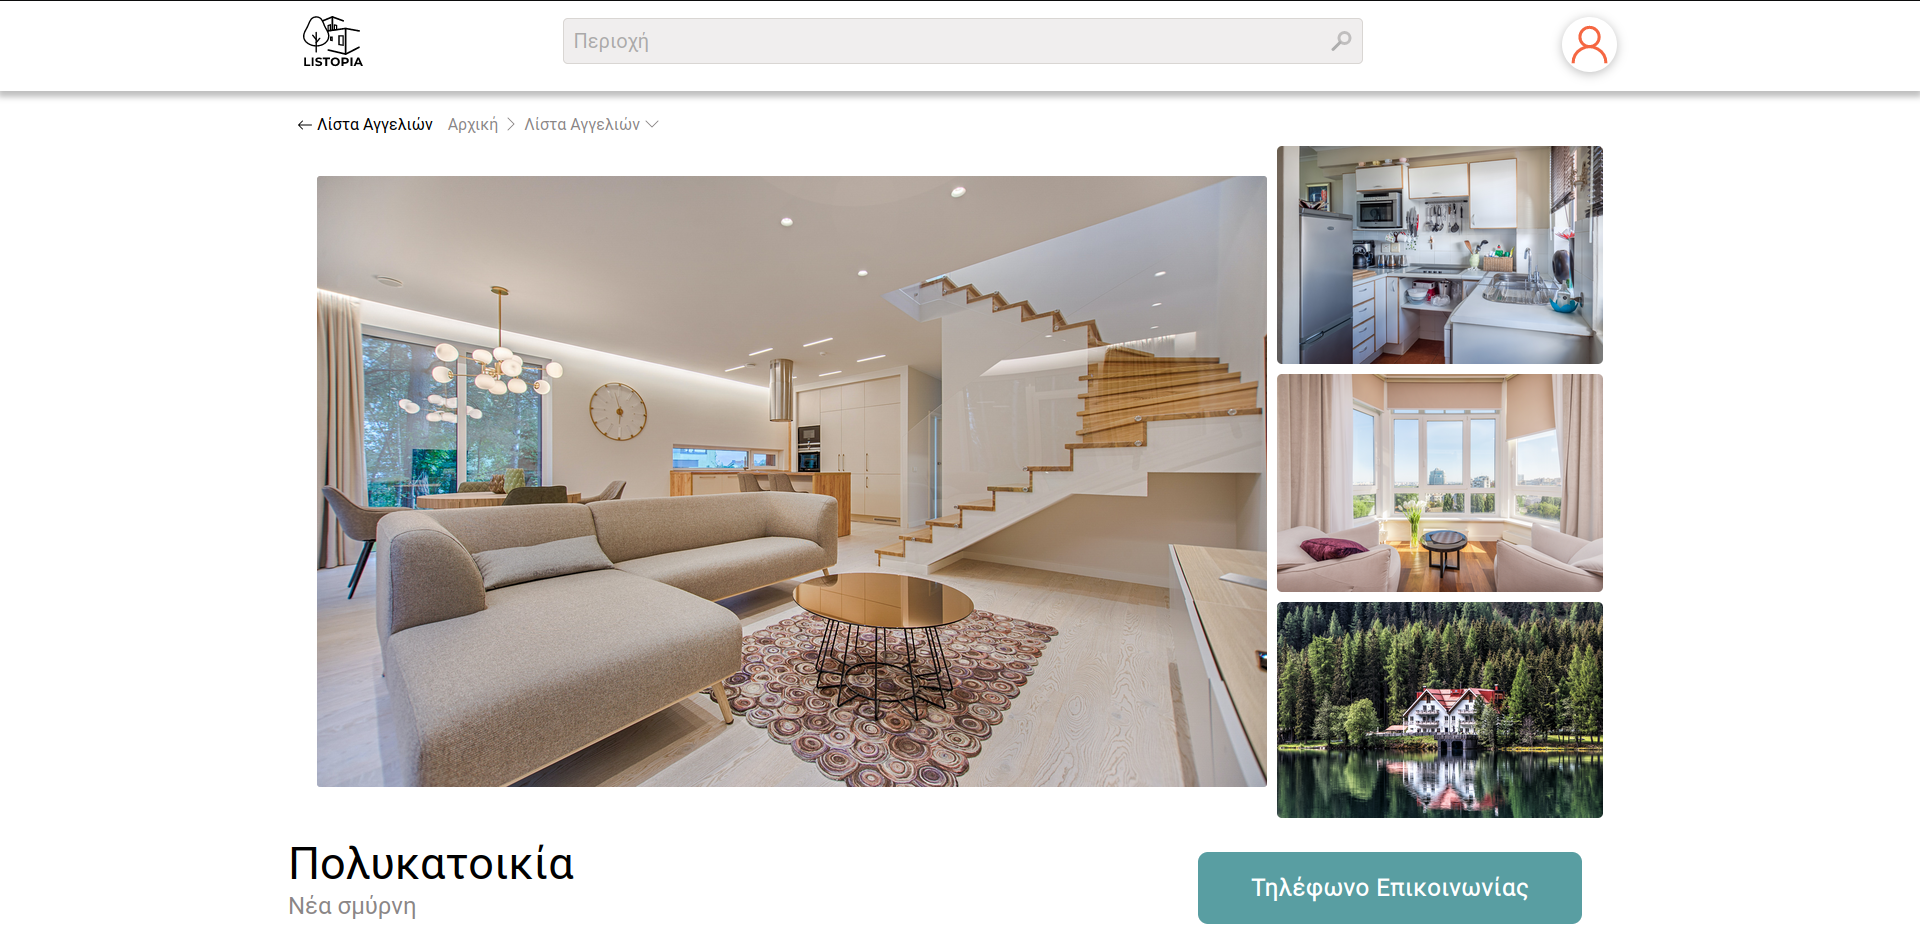
\includegraphics[width=\textwidth]{listing_page1.png}
		   \caption{Προεπισκόπηση εικόνων αγγελίας}
		   \label{fig:listing_preview}
	\end{figure}

	\begin{figure}[H]
		   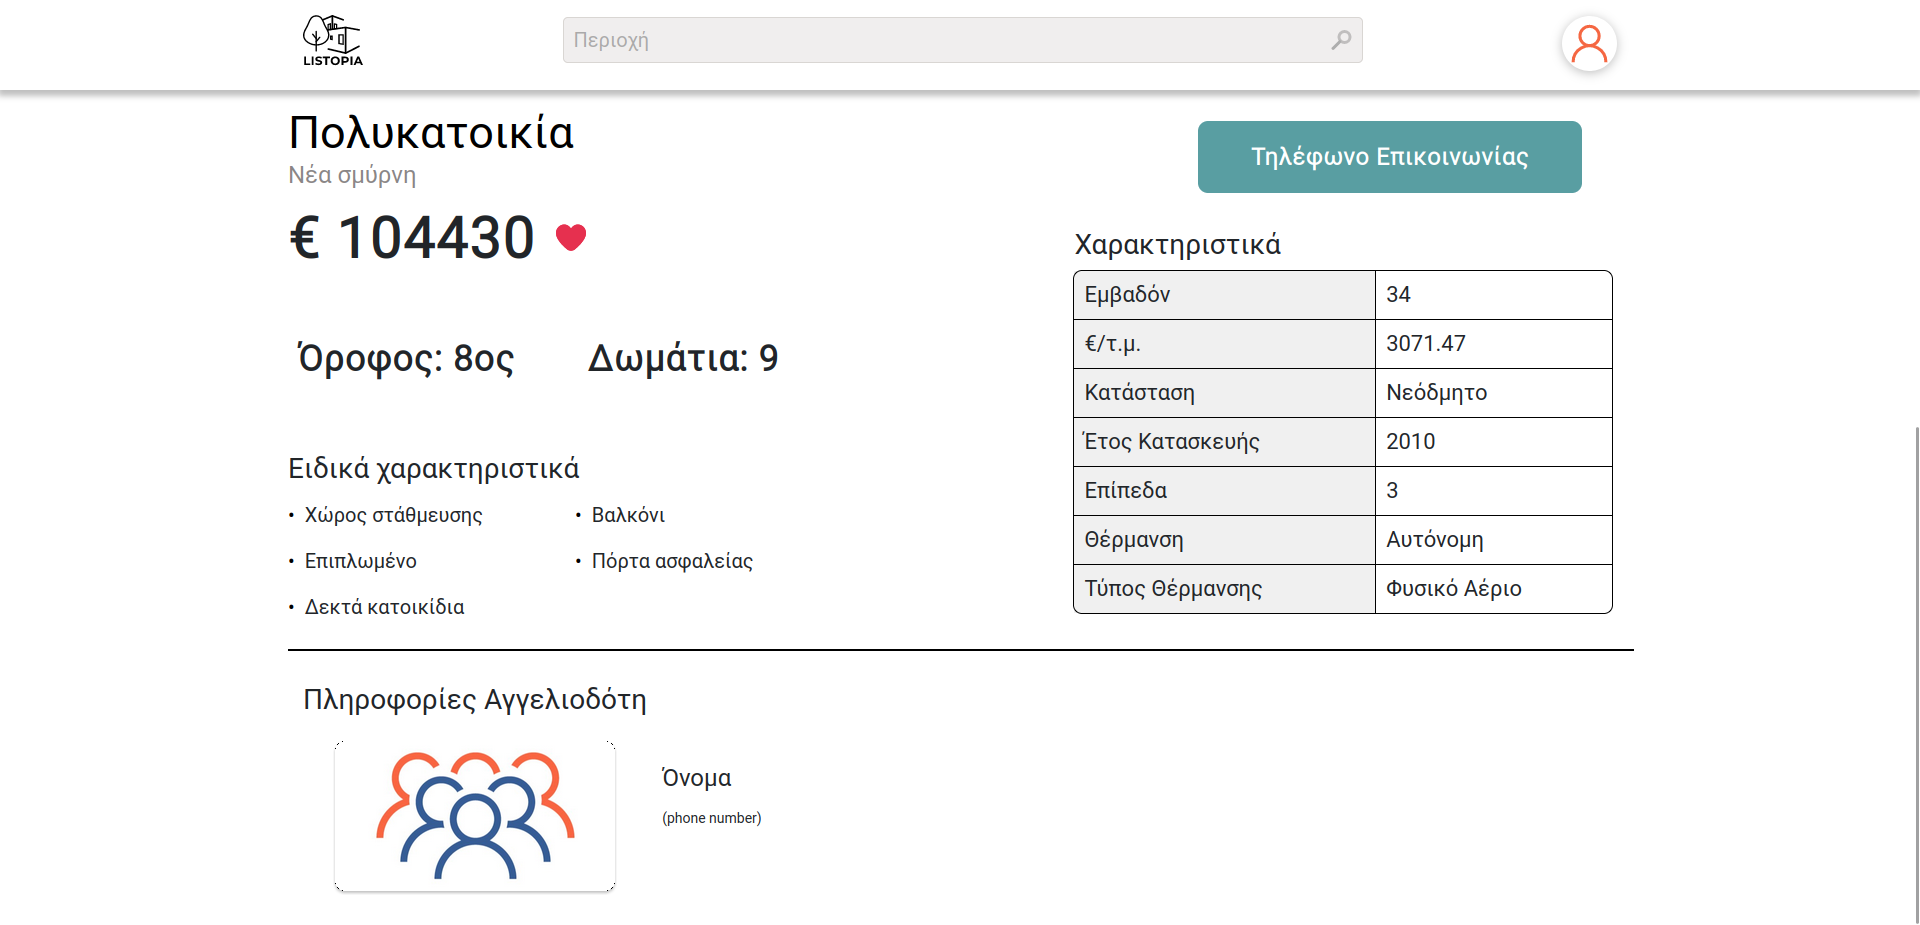
\includegraphics[width=\textwidth]{listing_page2.png}
		   \caption{Στοιχεία αγγελίας}
		   \label{fig:listing_info}
	\end{figure}

	\begin{figure}[H]
		   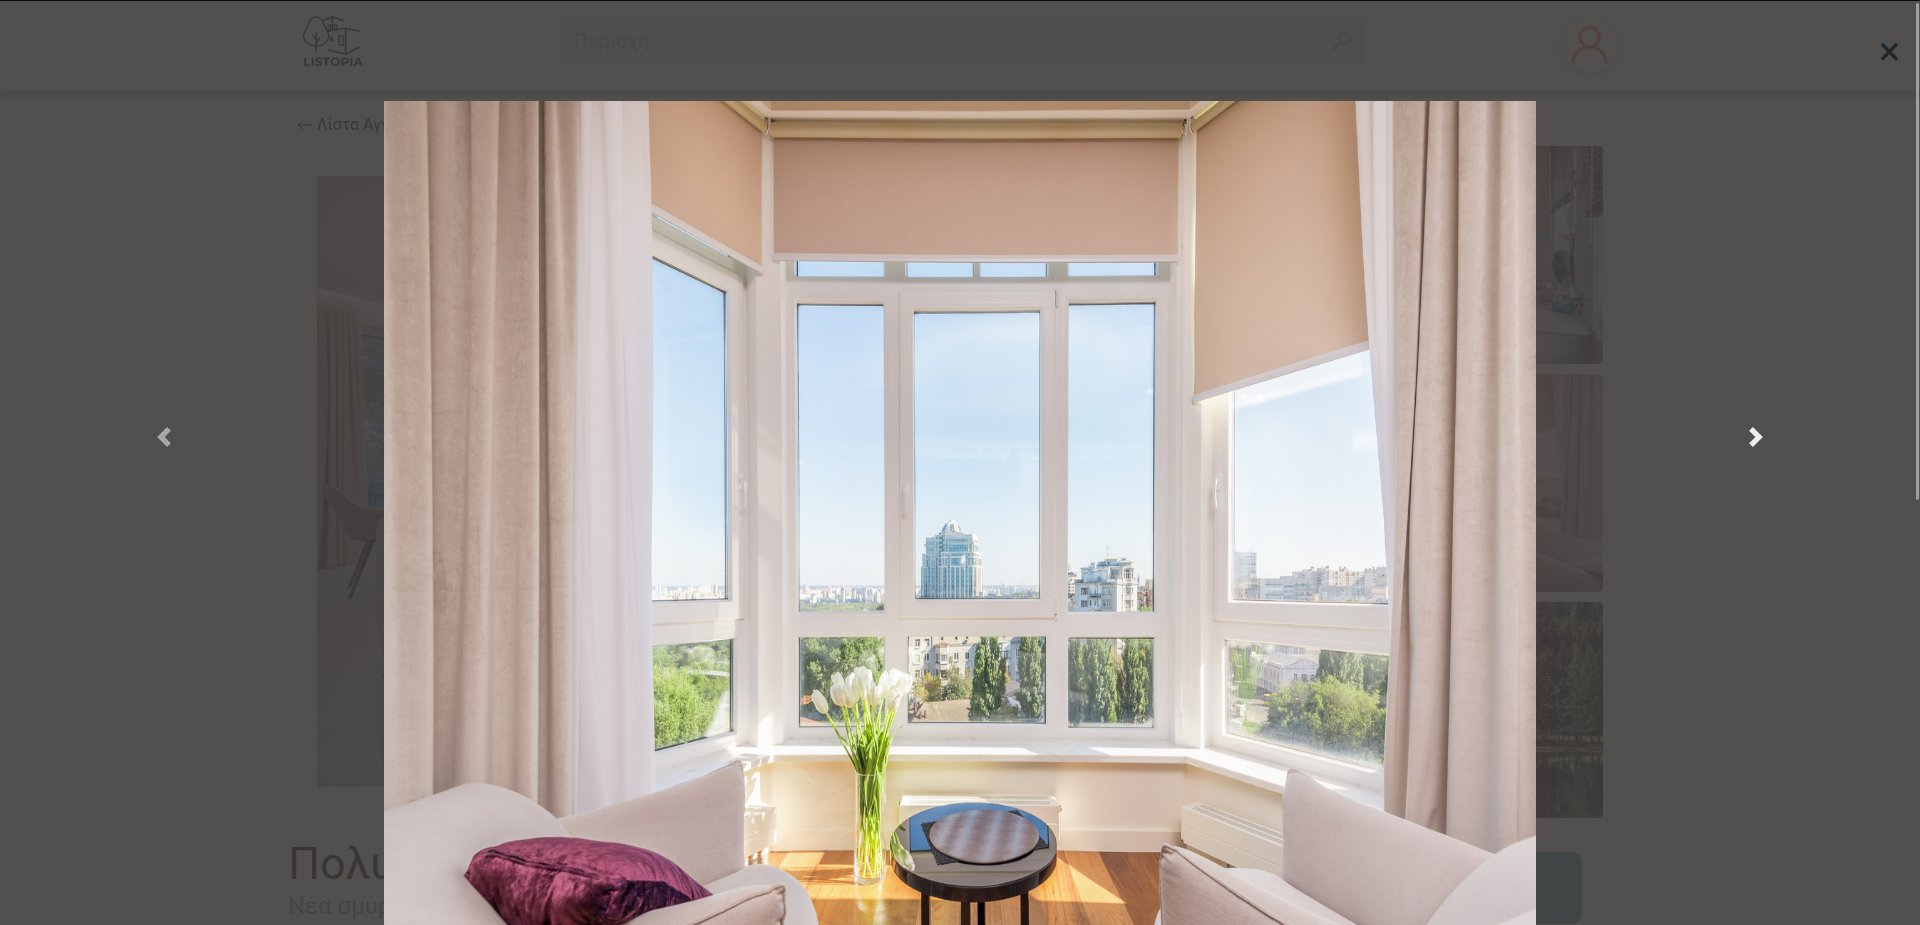
\includegraphics[width=0.8\textwidth]{listing_carousel.png}
		   \caption{Carousel Φωτογραφιών}
		   \label{fig:carousel}
	\end{figure}

\subsection{Σελίδες Εισόδου και Εγγραφής}
	Όσο αφορά την δημιουργία λογαριασμού στην εφαρμογή, ζητείται από τον χρήστη να
	συμπληρώσει κάποια απαραίτητα χαρακτηριστικά όπως μία διεύθυνση ηλεκτρονικού
	ταχυδρομίου, το όνομα του και τέλος τον κωδικό του όπως φαίνεται στην εικόνα
	\emph{\ref{fig:sign_up}}. Εφόσον γίνουν όλα αυτα επιτυχώς, είναι εφικτή η σύνδεση
	του στην σελίδα. Για την σύνδεση του, ζητείται η συμπλήρωση της διεύθυνσης
	ηλεκτρονικού ταχυδρομίου και κωδικός που υπέβαλλε κατά την εγγραφή του όπως φαίνεται
	και στην εικόνα \emph{\ref{fig:sign_in}}.

	\begin{figure}[H]
		   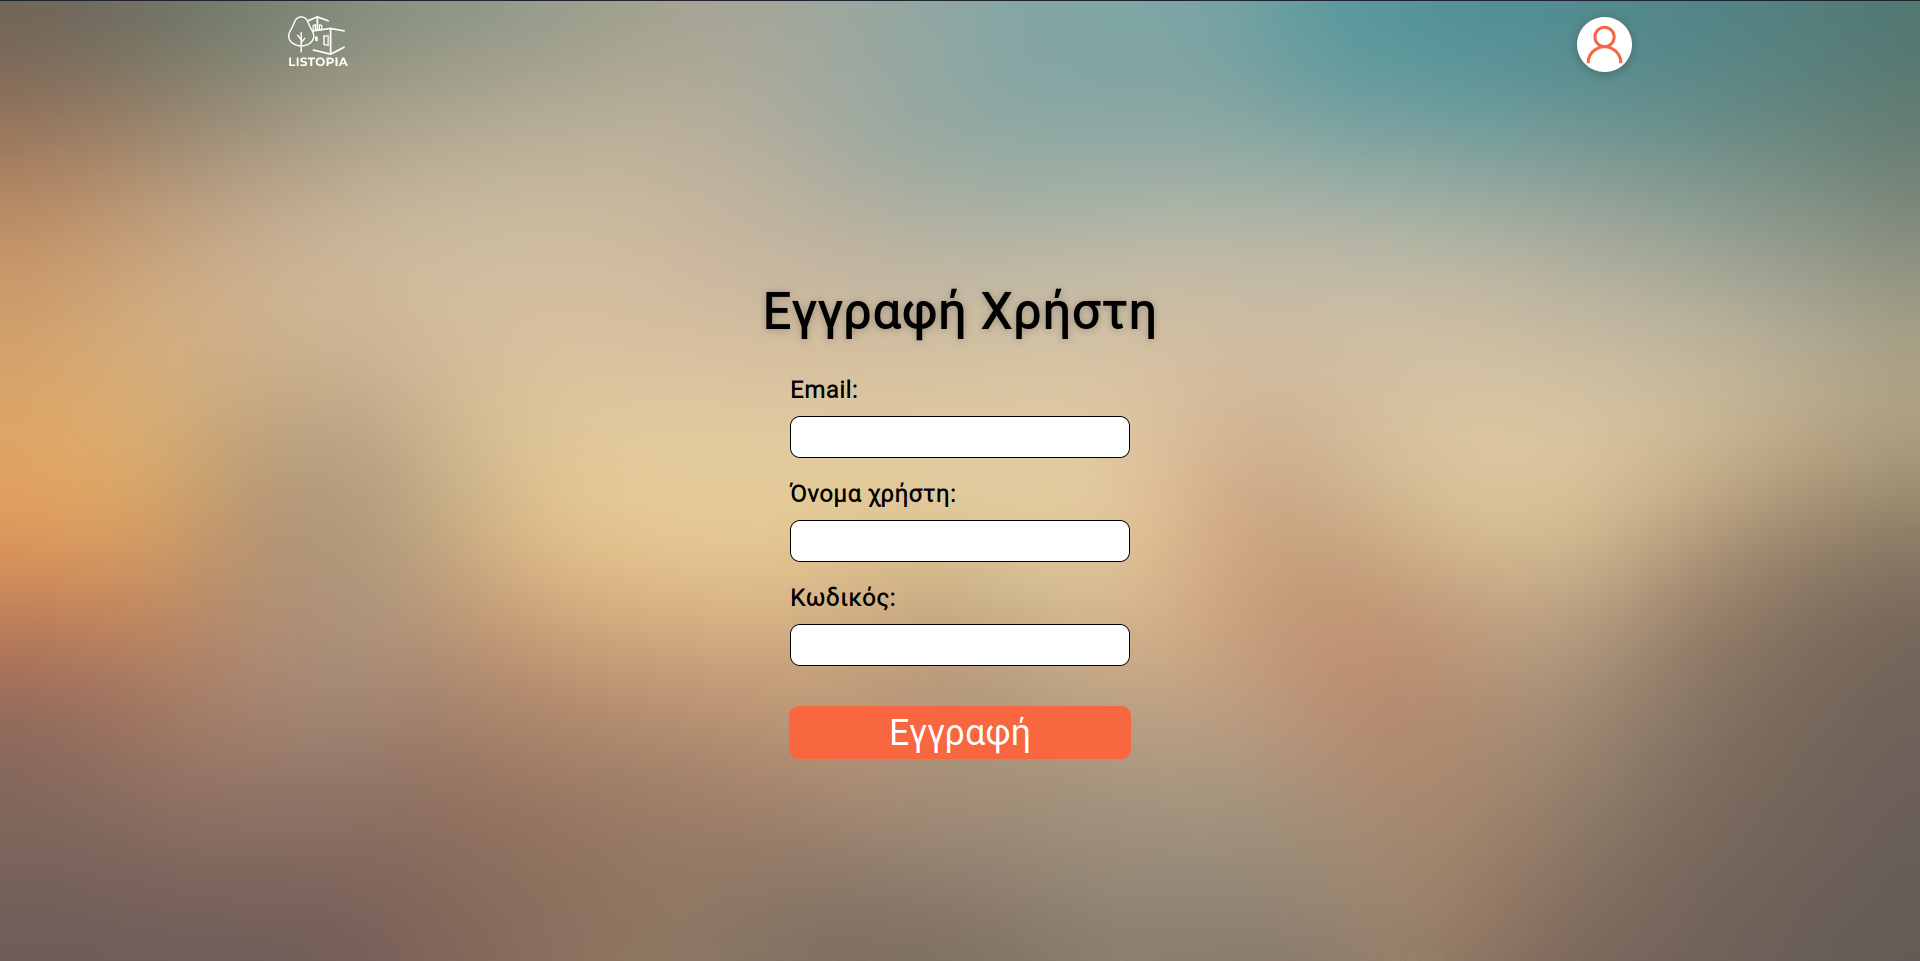
\includegraphics[width=0.8\textwidth]{sign_up_page.png}
		   \caption{Εγγραφή Χρήστη}
		   \label{fig:sign_up}
	\end{figure}

	\begin{figure}[H]
		   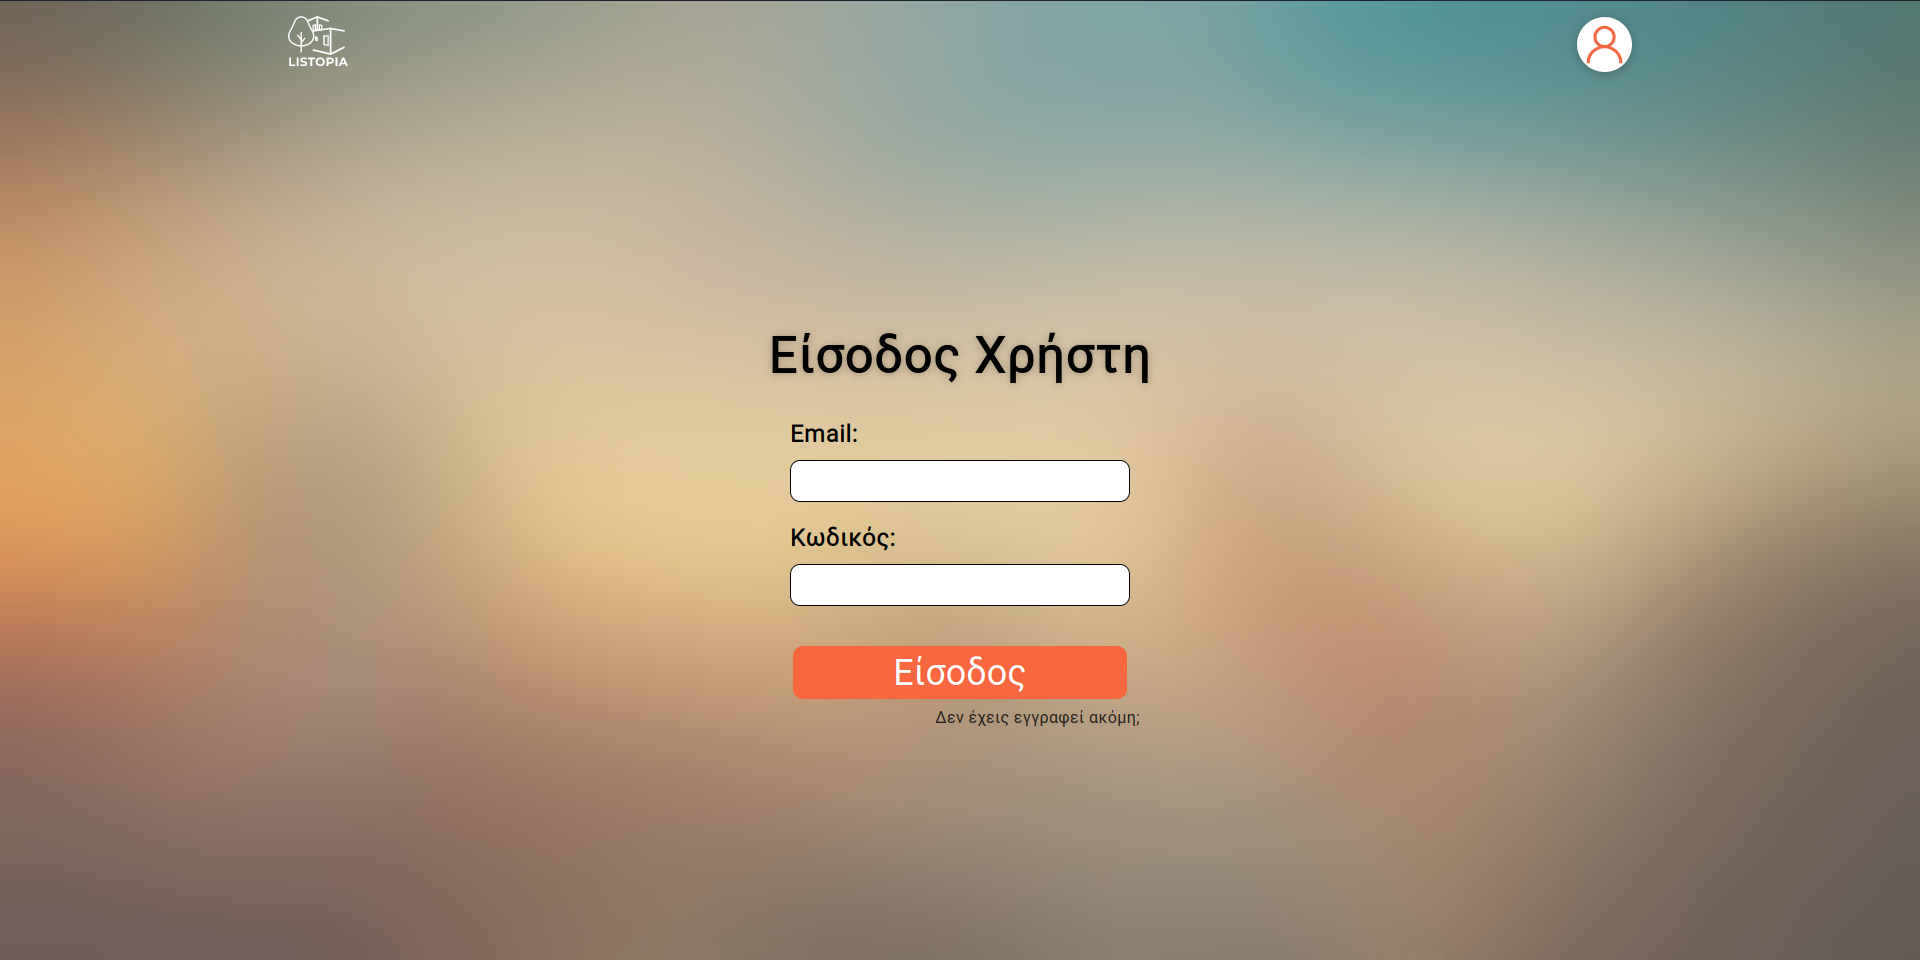
\includegraphics[width=0.8\textwidth]{sign_in_page.png}
		   \caption{Είσοδος Χρήστη}
		   \label{fig:sign_in}
	\end{figure}

\subsection{Σελίδα Προφίλ Χρήστη}
	Εφόσον ο χρήστης έχει συνδεθεί, στην σελίδα του Προφίλ του παρουσιάζονται τα στοιχεία
	που έχει συμπλήρώσει και του δίνεται η επιλογή να τα τροποποιήσει και να τα
	αποθηκεύσει. Επιπλέον, παρουσιάζονται σε μία λίστα όλες οι αγγελίες που ο χρήστης
	έχει επιλέξει ως αγαπημένες, εφόσον υπάρχουν.

	\begin{figure}[H]
		   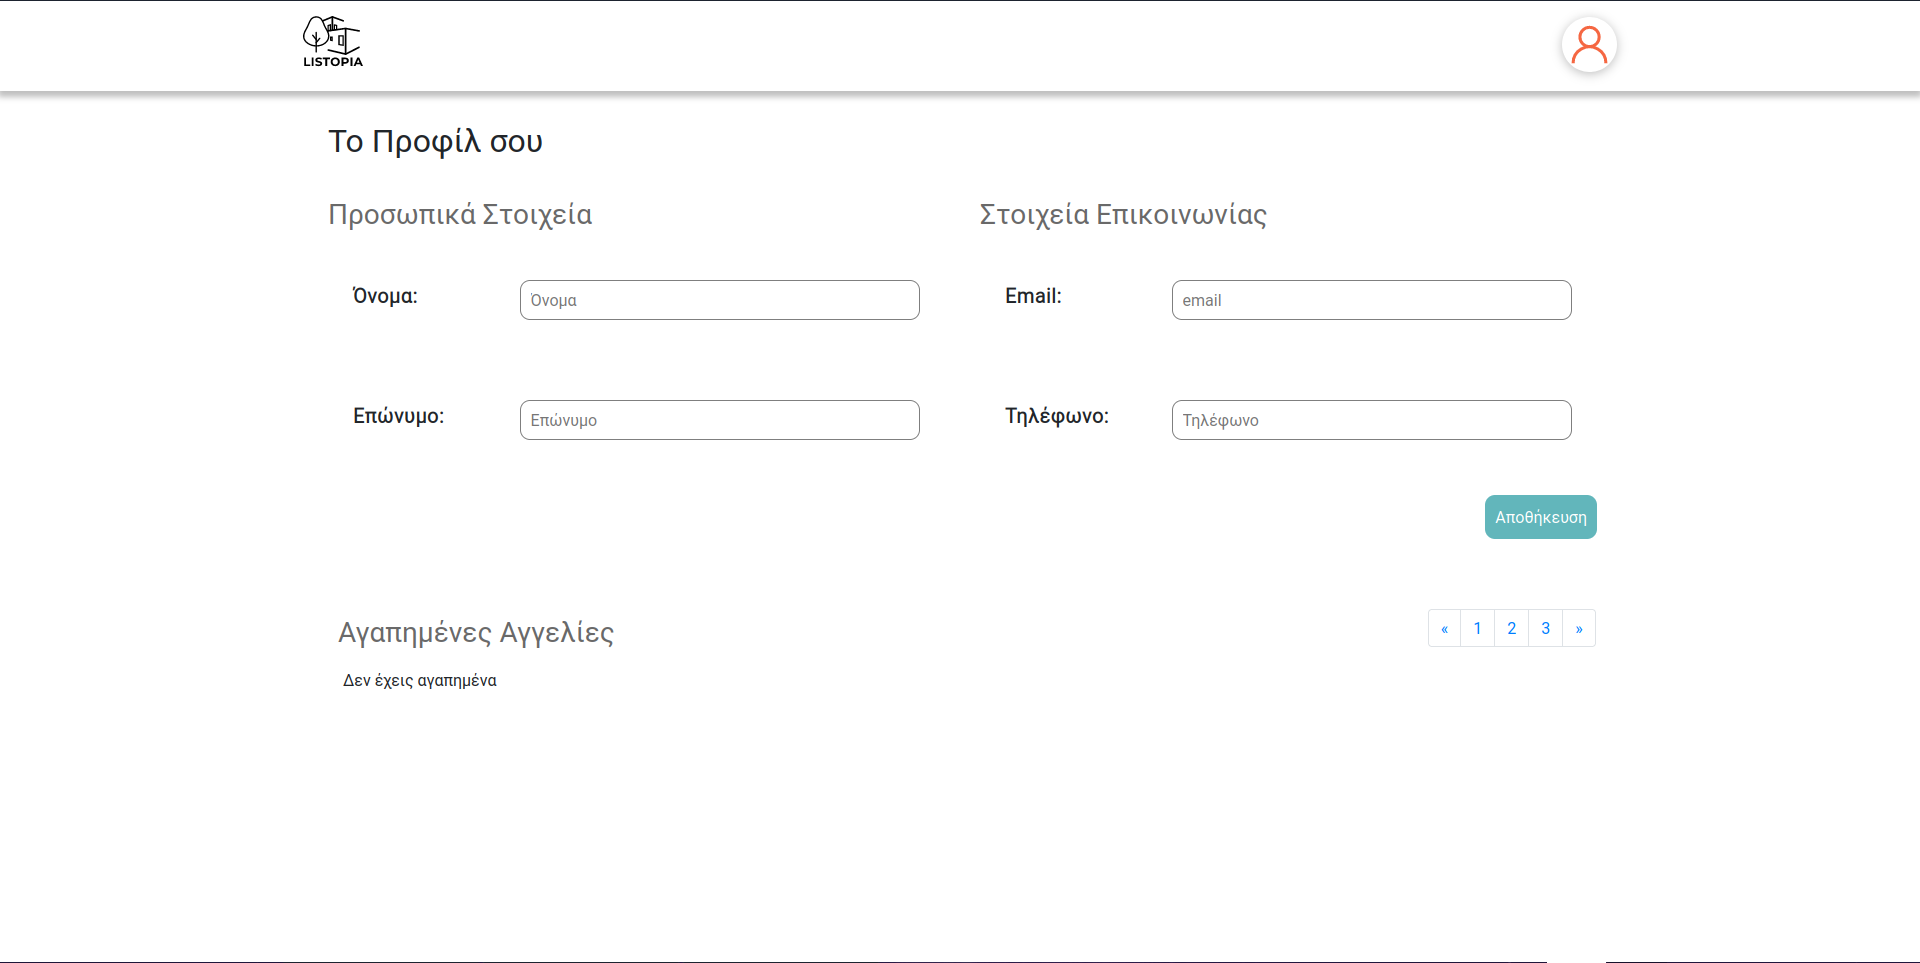
\includegraphics[width=0.8\textwidth]{profile_page.png}
		   \caption{Σελίδα Προφίλ Χρήστη}
		   \label{fig:profile}
	\end{figure}


\section{Backend}
\subsection{Σχεδίαση Βάσης Δεδομένων}
	Η ιστοσελίδα έχει την απαίτηση για αποθήκευση κάποιων δεδομένων. Συγκεκριμένα, αυτά
	τα δεδομένα είναι το σύνολο των αγγελιών και το σύνολο των χρηστών της ιστοσελίδας,
	καθώς και όλες οι πληφορίες που σχετίζονται με καθένα από αυτά. Για την αποθήκευση
	των δεδομένων απαιτείται μια κάποια βάση δεδομένων. Οι βάσεις δεδομένων χωρίζονται σε
	δύο βασικές κατηγορίες, τις σχεσιακές (SQL) και τις μη σχεσιακές (NoSQL). Επειδή τα
	δεδομένα της ιστοσελίδας είναι κατά κύριο λόγο ασυσχέτιστα μεταξύ τους, έγινε η
	επιλογή της βάσης δεδομένων MongoDB (που ειναι του τύπου NoSQL) καθώς αποθηκεύει
	τα δεδομένα σε μορφή παρόμοια με αρχείο JSON.

	Για τη δημιουργία των δεδομένων της ιστοσελίδας χρησιμοποιήθηκε το εργαλείο Mockaroo.
	Το εργαλείο αυτό μπορεί με κάποιες βασικές εντολές να παράξει μεγάλο πλήθος
	αληθοφανών δεδομένων, τα οποία όμως πολλές φορές δεν είναι ιδιαίτερα ρεαλιστικά.

\subsection{Βασική δομή Backend}
	Το Backend της ιστοσελίδας έχει δομηθεί με βάση το πρότυπο Model View Controller
	(MVC). Στο πρότυπο αυτό ορίζονται τα μοντέλα των δεδομένων (Model), η παρουσίαση των
	σελίδων (View) και η συμπεριφορά της εφαρμογής στα διάφορα αιτήματα του χρήστη
	(Controller). Για την καλύτερη οργάνωση του κώδικα, τα τρία αυτά κομμάτια του
	εξυπηρετητή έχουν τοποθετηθεί σε ξεχωριστά αρχεία και σε διαφορετικούς φακέλους.
	Ένα άλλο κομμάτι της οργάνωσης που δεν προκύπτει από το πρότυπο, είναι αυτό των
	διαδρομών (Routes) που καθορίζουν ποιο controller αντιστοιχεί στο κάθε αίτημα
	του χρήστη.

\subsection{Model}
	Η εφαρμογή έχει δύο είδη δεδομένων (της αγγελίες και τους χρήστες), οπότε έχει και
	δύο Models. Ένα Model περιγράφει τη μορφή των δεδομένων, δηλαδή τα πεδία που
	αποτελούν μια καταχώρηση στη βάση δεδομένων (π.χ για τους χρήστες το όνομα, το email
	κτλ). Ευθύνεται επίσης και για την άμεση σύνδεση του εξυπηρετητή με την βάση
	δεδομένων, καθώς και για τη "μετάφραση" των δεδομένων από τη μορφή στην οποία
	βρίσκονται αποθηκευμένα στη βάση, σε μια μορφή που είναι αξιοποιήσιμη από τον
	υπόλοιπο κώδικα.

\subsection{View}
	Σε κάθε σελίδα της εφαρμογής αντιστοιχεί και ένα αρχείο template της μορφής
	Handlebars το οποίο καθορίζει πως παρουσιάζεται αυτή στον χρήστη.
	Μέσω του εργαλείου Handlebars μπορεί πολύ εύκολα
	να προστεθούν στην HTML της σελίδας τα δεδομένα που προκύπτουν από τη βάση δεδομένων.
	Για την καλύτερη οργάνωση αυτού του κομματιού της εφαρμογής, πολλά κομμάτια κώδικα
	που επαναλαμβάνονται έχουν απομονωθεί σε διαφορετικά αρχεία (partials), όπως το
	κομμάτι της επικεφαλίδας (headers), και εισάγονται όπου είναι απαραίτητα. Την ώρα που
	μια σελίδα επρόκειτο να εμφανιστεί στο χρήστη, στο template εισάγονται τα δεδομένα
	που σχετίζονται με την σελίδα.

\subsection{Routes}
	Σε μια ιστοσελίδα υπάρχουν διάφορες λειτουργίες στις οποίες μπορεί να έχει πρόσβαση
	ο χρήστης. Για κάθε μία από αυτές τις λειτουργίες χρειάζεται ξεχωριστή δρομολόγηση,
	που καθορίζεται από το URL του αιτήματος. Οι διαδρομές της εφαρμογής ορίζονται μέσα
	από τα Routes, όπου κάθε Route ορίζει τη διαδομή και την μέθοδο HTTP στην οποία
	ανταποκρίνεται. Στη συνέχεια, το Route ορίζει την αλυσίδα των Controllers που θα
	επεξεργαστούν το αίτημα του χρήστη προκειμένου να προκύψει το κατάλληλο αποτέλεσμα.

\subsection{Controller}
	Για κάθε αίτημα του χρήστη πρέπει να εκτελεστούν κάποιες διαδικασίες για να
	εξυπηρετηθεί κατάλληλα. Για παράδειγμα αν ο χρήστης επιλέξει να αναζητήσει τις
	αγγελίες με βάση κάποια κριτήρια, πρέπει αυτά τα κριτήρια να αναγνωριστούν και να
	γίνει η αντίστοιχη αναζήτηση στη βάση δεδομένων και τα αποτελέσματα να εμφανιστούν.
	Κάθε μία από αυτές τις διαδικάσιες εκτελείται από ένα Controller στην αλυσίδα, το
	οποίο διαβάζει τα δεδομένα του αιτήματος και τα επεξεργάζεται αντιστοίχως μέχρις
	ότου να σταλεί το αποτέλεσμα στον χρήστη.


\subsection{Διαδικασία Εξουσιοδότησης}
	Πολλές από τις λειτουργίες της ιστοσελίδας αφορούν έναν χρήστη συγκεκριμένα. Οπότε
	είναι απαραίτητο πριν επιτραπεί η πρόσβαση σε αυτές να επιβεβαιωθεί η ταυτότητα του
	χρήστη, ή αλλιώς να εξουσιοδοτηθεί ο χρήστης. Για κάθε Route της εφαρμογής που
	απαιτείται εξουσιοδότηση λέγεται ότι βρίσκεται στη ασφαλή περιοχή (secure area). Άρα
	προστίθεται ένας επιπλέον Controller στην αλυσίδα εξυπηρέτησης όπου ελέγχεται αν το
	αίτημα προέρχεται από χρήστη που του έχουν παραχωρηθεί τα κατάλληλα δικαιώματα. Αν ο
	προηγούμενος έλεγχος είναι επιτυχής, το αίτημα προχωράει για εξυπηρέτηση από το
	Controller που του αντιστοιχεί, αλλιώς ο χρήστης παραπέμπτεται στην σελίδα Sign In.
	Στη σελίδα Sign In ο χρήστης έχει την επιλογή να συνδεθεί με τα στοιχεία του, αλλιώς
	αν είναι νέος χρήστης μπορεί να πλοηγηθεί στη σελίδα Sign Up, όπου θα συμπληρώσει όλα
	τα απαραίτητα στοιχεία προκειμένου να δημιουργηθεί μια καινούρια εγγραφή στη βάση
	δεδομένων.

\subsection{Διαχείρηση Συνεδριών}
	Αφού συνδεθεί ένας χρήστης στην ιστοσελίδα, είναι χρήσιμο να διατηρείται η σύνδεση
	του και για μεταγενέστερα αιτήματα, αντί να πρέπει να συνδέεται κάθε φορά που
	προσπαθεί να εισέλθει στην ασφαλή περιοχή. Για τον σκοπό αυτό έχει υλοποιηθεί σύστημα
	διαχείρισης συνεδρίας (session control), μέσω του εργαλείου express-session. Έτσι
	όταν ο χρήστης εξουσιοδοτείται, αποθηκεύεται στην μεριά του ένα cookie που πιστοποιεί
	τη συγκεκριμένη συνεδρία και παραπέμπει τον εξυπηρετητή σε κάποια αποθηκευμένα
	δεδομένα αναφορικά με την ταυτότητα του χρήστη. Οι συνεδρίες έχουν χρονικό όριο
	διάρκειας 90 λεπτών, μετά το πέρας αυτού ο χρήστης θα πρέπει να ξανασυνδεθεί.

\bibliography{bibliography}


\appendix

\section{Οδηγίες εγκατάστασης της εφαρμογής}
	Η ανάπτυξη της ιστοσελίδας έγινε με τη βοήθεια του εργαλείου Docker το οποίο σημαίνει
	πως για να εγκατασταθεί η εφαρμογή σε κάποιο εξυπηρετητή αρκεί μόνο να είναι
	εγκατεστημένο το περιβάλλον Docker και να εκτελεστεί η εντολή

	docker compose up --build -d




\end{document}
\endinput
